% +--------------------------------------------------------------------+
% | Sample Chapter 2
% +--------------------------------------------------------------------+

\cleardoublepage

% +--------------------------------------------------------------------+
% | Replace "This is Chapter 2" below with the title of your chapter.
% | LaTeX will automatically number the chapters.
% +--------------------------------------------------------------------+

\chapter{OpenGL y DirectX}
\label{makereference2}

El objetivo de este capítulo es explicar en qué consiste OpenGl, así como su
pipeline de gráficos, los tipos de shaders que incluye y las diferencias que
presenta con DirectX, su principal competidor.\\

\section{¿Qué es?}
\label{makereference2.1}

OpenGL se define como una API \textit{(application programming interface)}, que
es simplemente una librería de software para acceder a capacidades del hardware
de gráficos (ver \citet{Shreiner:2009:OPG:1696492}).

OpenGL está diseñado como una interfaz independiente del hardware que puede ser
implementada en muchos sistemas hardware de gráficos diferentes, o completamente
como software, en el caso de que el sistema no posea hardware de gráficos.
OpenGL no proporciona ninguna funcionalidad para describir modelos en tres
dimensiones ni operaciones para leer ficheros (como imágenes JPEG, por ejemplo).
En su lugar, se deben construir los objetos tridimensionales a partir de un
pequeño conjunto de primitivas geométricas---puntos, líneas, triángulos y
parches. 

\section{Breve historia de OpenGL}
\label{makereference2.2}

OpenGL nace a principios de los años 90, desarrollada por Silicon Graphics~(SGI).  En
los años 80, Silicon Graphics poseía una API privada denominada IRIS GL,
utilizada para producir gráficos en sus estaciones de trabajo IRIS.
Posteriormente, debido a la pérdida de cuota de mercado, decidió hacer su API
pública. Sin embargo, a causa de problemas con patentes y el hecho de tener
características poco relevantes para los gráficos 3D como la funcionalidad de
ventanas, se decidió reescribir algunas de las partes y se lanzó lo que ahora se
conoce como OpenGL.\\

Esta nueva especificación consiguió logros importantes para la informática gráfica,
como estandarizar el acceso al hardware gráfico, trasladar a los fabricantes la
responsabilidad del desarrollo de las interfaces con el hardware y delegar la
funcionalidad de ventanas al sistema operativo. Todo esto supuso un gran impacto
en la industria, al ofrecer a los desarrolladores una plataforma de alto nivel
sobre la que trabajar.\\

En 1992, Silicon Graphics lideró la creación del OpenGL Architecture Review
Board (OpenGL ARB)~\cite{OpenGLARB}, un grupo de empresas del sector que sería la encargada de
mantener y extender la especificación en los años siguientes. El OpenGL ARB
estaba formado por 3Dlabs, Apple, ATI, Dell, IBM, Intel, Nvidia, SGI and Sun
Microsystems.\\

En otoño de 2006, el OpenGL ARB y los directores de Khronos votaron para transferir el
control de OpenGL a Khronos Group. El secretario de la ARB Jon Leech observó:
\textit{"Hemos decidido mover OpenGL a Khronos para asegurar la salud futura de
OpenGL en todas sus formas."}\cite{OpenGLARB}

\section{Diseño}
\label{makereference2.3}

\begin{figure}[h]%t=top, b=bottom, h=here

	\begin{center}
	    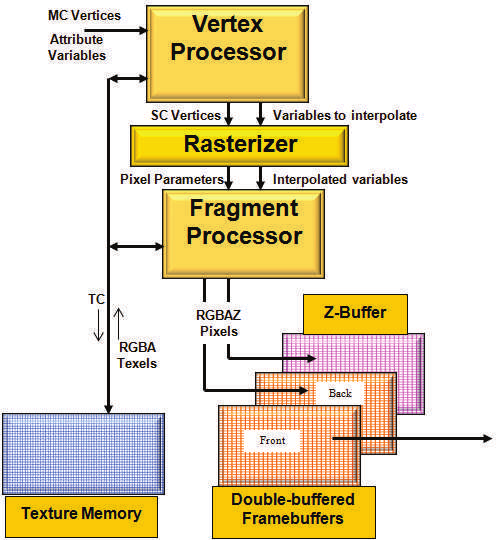
\includegraphics[height=4in]{figures/pipeline.png}
	    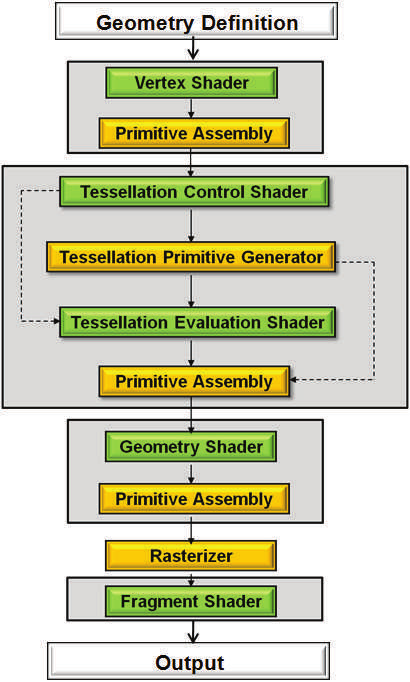
\includegraphics[height=4in]{figures/pipelineExtendido.png}
	\end{center}

    \caption[Pipeline de OpenGl]{Pipeline de OpenGl en el hardware gráfico.}
	\label{figurePipeline}

\end{figure}



% +--------------------------------------------------------------------+
% | In this chapter, I want to refer to Chapter~\ref{makereference},
% | so I'm going to use the slash ref command along with the
% | "makereference" label which I assigned back at the beginning of
% | Chapter 1.
% | 
% | \section{Page Number References}
% | \label{makereference2.1} I should also be able to refer to a
% | specific page number, such as page~\pageref{makereference}.  Of
% | course, I'll need to have a slash label command and a unique name
% | in each section that I want to be able to refer to later in the
% | text.
% | 
% | \section{Referring to Sections Within Chapter 1}
% | \label{makereference2.2} Now, I'm going to refer to different
% | sections within Chapter 1. I gave an example of a figure in
% | section~\ref{makereference1.1} and an example of a table in
% | section~\ref{makereference1.2}.  In
% | section~\ref{makereference1.3}, we looked at examples of
% | bibliographic citations.
% +--------------------------------------------------------------------+
